\section{eo\-Eval\-Func\-Counter$<$ EOT $>$ Class Template Reference}
\label{classeo_eval_func_counter}\index{eoEvalFuncCounter@{eoEvalFuncCounter}}
Counts the number of evaluations actually performed, thus checks first if it has to evaluate..  


{\tt \#include $<$eo\-Eval\-Func\-Counter.h$>$}

Inheritance diagram for eo\-Eval\-Func\-Counter$<$ EOT $>$::\begin{figure}[H]
\begin{center}
\leavevmode
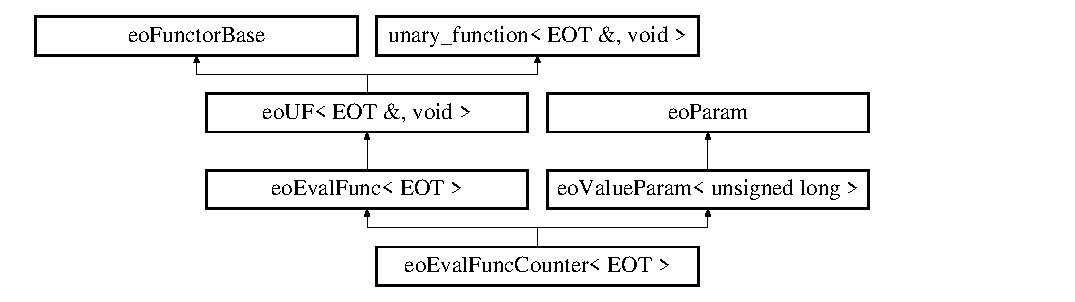
\includegraphics[height=3.60709cm]{classeo_eval_func_counter}
\end{center}
\end{figure}
\subsection*{Public Member Functions}
\begin{CompactItemize}
\item 
{\bf eo\-Eval\-Func\-Counter} ({\bf eo\-Eval\-Func}$<$ {\bf EOT} $>$ \&\_\-func, std::string \_\-name=\char`\"{}Eval. \char`\"{})\label{classeo_eval_func_counter_a0}

\item 
virtual void {\bf operator()} ({\bf EOT} \&\_\-eo)\label{classeo_eval_func_counter_a1}

\begin{CompactList}\small\item\em The pure virtual function that needs to be implemented by the subclass. \item\end{CompactList}\end{CompactItemize}
\subsection*{Private Attributes}
\begin{CompactItemize}
\item 
{\bf eo\-Eval\-Func}$<$ {\bf EOT} $>$ \& {\bf func}\label{classeo_eval_func_counter_r0}

\end{CompactItemize}


\subsection{Detailed Description}
\subsubsection*{template$<$class EOT$>$ class eo\-Eval\-Func\-Counter$<$ EOT $>$}

Counts the number of evaluations actually performed, thus checks first if it has to evaluate.. 

etc. 



Definition at line 37 of file eo\-Eval\-Func\-Counter.h.

The documentation for this class was generated from the following file:\begin{CompactItemize}
\item 
eo\-Eval\-Func\-Counter.h\end{CompactItemize}
